\chapter{Segmentación de imágenes con base en color}

	En este capítulo se desarrollan los conceptos necesarios para entender la visión computacional que se empleará en este trabajo. Comenzando con definiciones importantes y entendiendo cómo es que funcionan las cámaras, con sus capacidades y limitaciones.
	
	Dentro de la sección 3.2 se describen lo modelos matemáticos para corregir las diversas distorsiones que una cámra puede generar al momento de tomar una imagen (debido a sus irregularidades en la manufactura de las lentes).

	Por último se explica el método de segmentación basado en color, tomando como base el espacio de color HSV (más conveniente que el convencional RGB) y los métodos matemáticos para la eliminación de ruido, más comunmente conocidos como operadores morfológicos.
	
	\section{Modelo de cámara Estenopeica \textit{(Pinhole)}}

De acuerdo con \cite{bradski2008learning} la visión es la detección de la luz del mundo. El proceso de visión empieza cuando un rayo de luz es emanado desde una fuente hacia un objeto. Cuando la luz choca con el objeto, mucha de esta luz es absorbida, la que no, se puede percibir como el color, de esta manera, la luz reflejada hace su camino hacia el sensor óptico.

El modelo más simple de cómo sucede la captura de luz, es el de la cámara estenopeica o \textit{pinhole}. Una cámara estenopeica se puede imaginar como una habitación sin ventanas en donde la luz únicamente entra por una pequeña apertura en el centro de la pared proyectando así una imagen dentro de la habitación. Véase la Figura(\ref{fig:pinholeCamera}).

\begin{figure}
	\centering		
	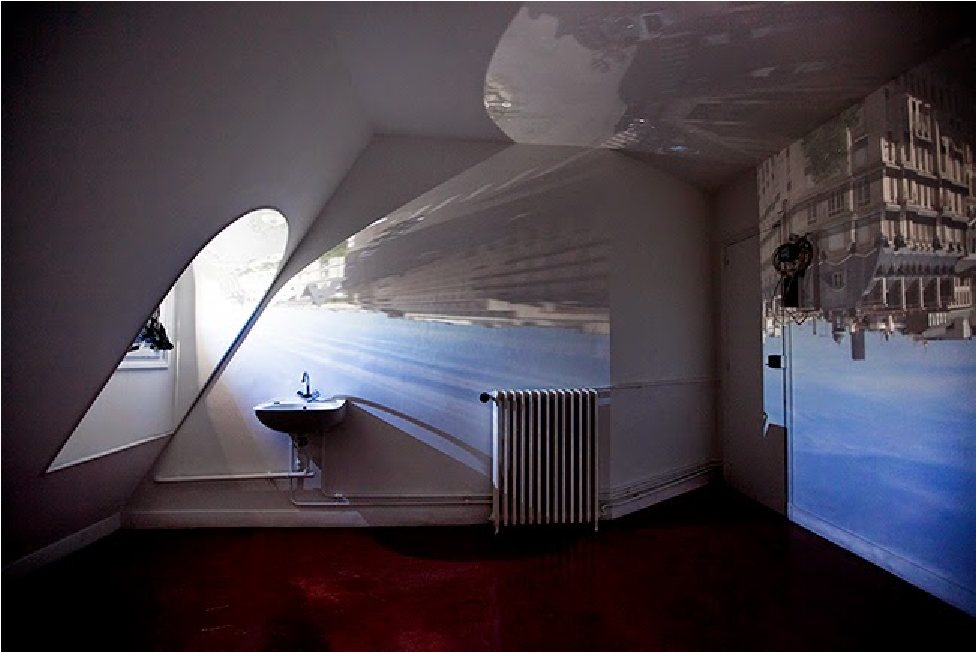
\includegraphics[scale=0.7]{images/pinholeCamera.pdf}
	\caption{Ejemplo en la vida real de la proyección de una imagen con la cámara estenopéica. Imagen tomada de: https://www.pinterest.com.mx/pin/371828512962028619.}		
	\label{fig:pinholeCamera}
\end{figure}

En la cámara estenopeica se considera que sólo un rayo de luz entra desde un punto en particular, este punto es luego \textit{proyectado} sobre una superficie generalmente plana. Como resultado, la imagen en este plano (también llamado plano proyectivo), está siempre en el foco y su tamaño se relaciona a la distancia del objeto por un sólo parámetro: \textit{la distancia focal}. La principal diferencia entre la imagen real y la que aparece en una cámara Pinhole, es que la imagen aparece invertida. 
	
El punto dentro del Pinhole es reinterpretado como el centro de proyección. Para este tipo de cámara, la distancia desde la abertura del Pinhole hacia la pantalla, es precisamente la distancia focal. Como puede verse en la Figura \ref{fig:pinholeScheme}.\\
	
\begin{figure}
	\centering		
	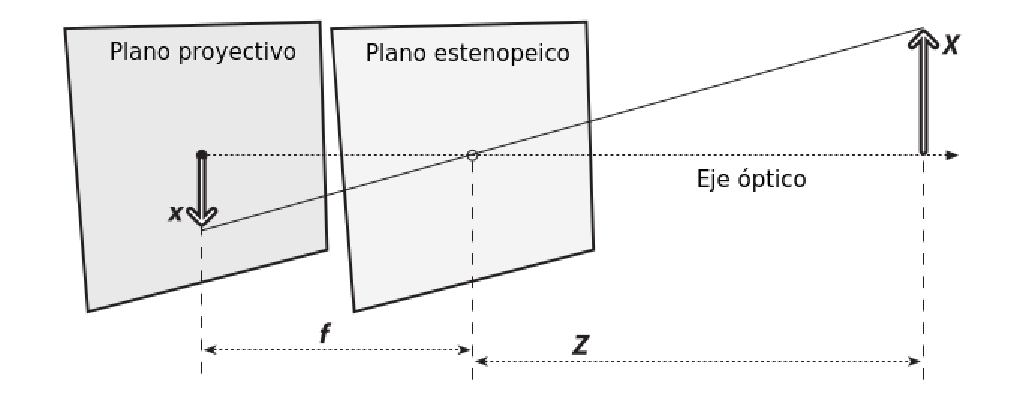
\includegraphics[scale=0.8]{images/pinholeScheme.pdf}
	\caption{Esquema del modelo de cámara estenopeica. Imagen modificada de: \cite{bradski2008learning}.}		
	\label{fig:pinholeScheme}
\end{figure}

En la Figura(\ref{fig:pinholeScheme}), $f$ es representada como la distancia focal de la cámara, $Z$ es la distancia de la cámara al objeto, $X$ es la longitud del objeto, y $x$ es la longitud de la la imagen proyectada en el plano. Dentro de la figura, se pueden ver dos triángulos semejantes de los cuales se puede deducir la siguiente expresión:
\[x = -f \frac{X}{Z}\]
	
Para fines prácticos, el modelo \textit{Pinhole} no es conveniente de usar en exposiciones rápidas, ya que toda su luz proviene de un solo punto. A fin de obtener otro modelo de cámara que recopile mayor cantidad de luz y tenga ecuaciones similares, pero sin signos negativos (correspondientes a la inversión de la imagen) se propone hacer un rearreglo en el que se coloca al frente del centro de proyección el plano proyectivo. Tal y como se ve en la Figura \ref{fig:rearrange_pinhole_scheme}.
	
\begin{figure}
	\centering
	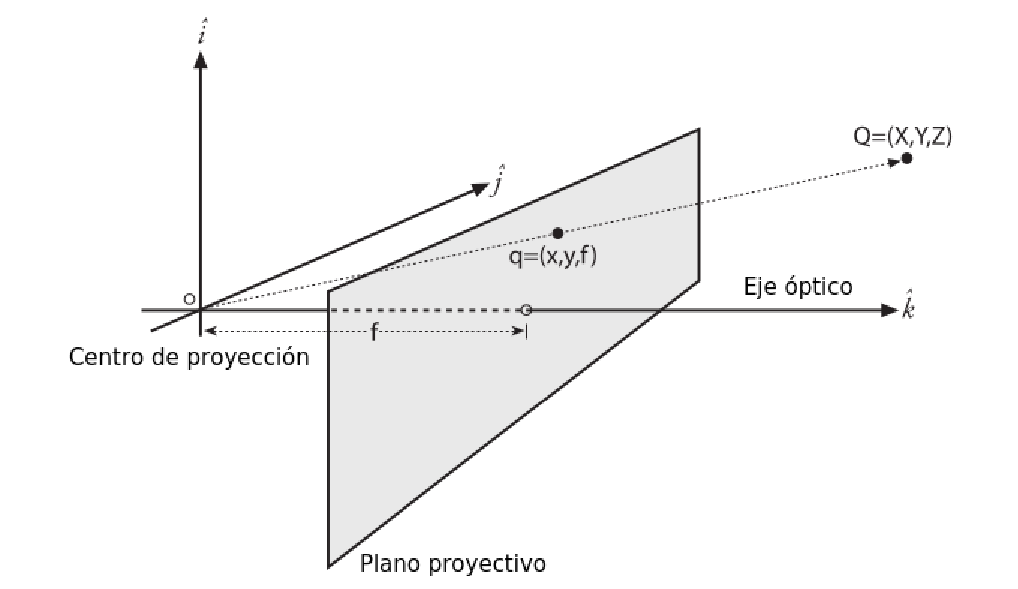
\includegraphics[scale=0.8]{images/rearrange_pinhole_scheme.pdf}
    \caption{Rearreglo de una cámara estenopeica. Imagen modificada de: \cite{bradski2008learning}.}
    \label{fig:rearrange_pinhole_scheme}
\end{figure} 

Con este nuevo cambio, cada rayo de luz proveniente del objeto distante se dirije hacia el \textit{centro de proyección} y deja un punto en el \textit{plano proyectivo}. El punto de intersección del plano proyectivo y el eje óptico es conocido como \textit{el punto principal}. La imagen proyectada en este nuevo plano de imagen, tiene exactamente el mismo tamaño que en el esquema mostrado en la Figura(\ref{fig:pinholeScheme}) pero en este caso, la imagen no queda invertida, por lo que su relación de triángulos quedaría de la siguiente manera: 

\[\frac{x}{f} = \frac{X}{Z}\]

Se podría pensar que que \textit{el punto principal} es equivalente al centro de la imagen, sin embargo, este centro usualmente no está en el eje óptico, es por eso que se introducen dos nuevos parámetros, $c_{x}$ y $c_{y}$ para modelar un posible desplazamiento (perpendicular al eje óptico) del centro de coordenadas en el plano de proyección. El resultado es que un punto $Q$ en el mundo físico cuyas coordenadas son  (X,Y,Z) es proyectado dentro de la pantalla en una localización de pixeles dada por $(x_{screen},y_{screen})$ de acuerdo con las siguientes ecuaciones:

\[x_{screen}=f_{x}\left(\frac{X}{Z}\right ) + c_{x}\]	
\[y_{screen}=f_{y}\left(\frac{Y}{Z}\right ) + c_{y}\]

Nótese que se han introducido dos diferentes distancias focales $f_{x}$ y $f_{y}$, la razón es porque generalmente los pixeles son rectangulares.
		
	\section{Corrección de la distorsión}
		\subsection*{Geometría básica proyectiva}
La relación que mapea los puntos $Q_{i}$ en el mundo físico con coordenadas $(X_{i},Y_{i},Z_{i})$ a los puntos en el plano de proyección con coordenadas $(x_{i},y_{i})$ es llamada una \textit{transformación proyectiva}. Cuando se trabaja con estas transformaciones es conveniente usar las \textit{coordenada homogéneas}. El plano de imagen es el espacio proyectado y tiene dos dimensiones, con lo que se pueden representar puntos en el plano como un vector tridimensional $q=(q_{1},q_{2},q_{3})$ ó $q=(x, y, w)$, en donde w es la orientación. Una forma de hacer un arreglo con los parámetros que definen a la cámara $f_{x},f_{y},c_{x}$ y $c_{y}$ dentro de una matriz de 3x3 es la llamada \textit{matriz de parámetros intrínsecos}. La proyección $q$ de los puntos del mundo físico en el plano de la imagen se puede calcular como: 
\[q=MQ\]
donde
\[q=
\begin{bmatrix}
x\\ 
y\\
w 
\end{bmatrix}\;,\;M=
\begin{bmatrix}
f_{x} & 0 & c_{x}\\ 
0     &f_{y}&c_{y} \\
0     & 0 & 1
\end{bmatrix}\;,\;Q=
\begin{bmatrix}
X\\
Y\\
Z
\end{bmatrix}
\]
		\subsection*{Distorsión de las lentes}
Debido a diversos factores en la manufactura, las lentes de una cámara no son perfectas, y al obtener una imagen, esta puede notarse distorsionada (véase la Figura \ref{fig:image_distorted}). La distorsión es un fenómeno que todas las cámaras tienen, no obstante, es más evidente en las cámaras de baja calidad o en las que tienen lentes tipo \textit{ojo de pescado}. Las distorsiones más características son: las \textit{Distorsiones radiales} y las \textit{Distorsiones tangenciales}. Las primeras surgen como resultado de la forma de las lentes y las segundas como resultado del proceso de ensamblado de la cámara.

\begin{figure}
\centering
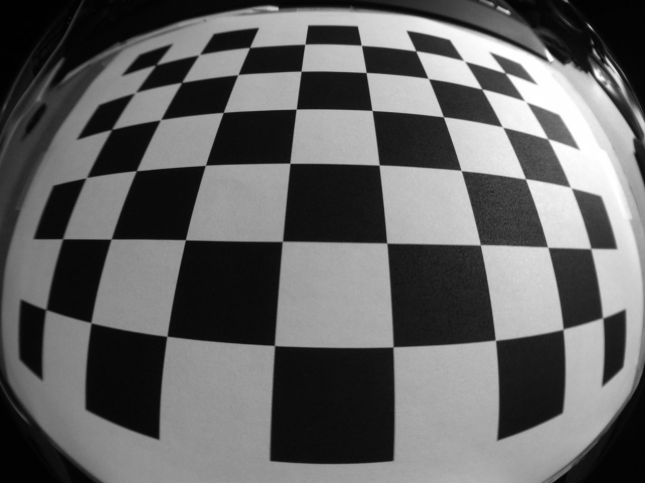
\includegraphics[scale=0.5]{images/image_distorted.png}
\caption{Ejemplo de distorsión de una cámara. Imagen tomada de: https://answers.opencv.org/question/114056/chessboard-detection-fails-on-fisheye-image/?sort=votes}
\label{fig:image_distorted}
\end{figure}

Cuando la imagen se hace más pequeña conforme está más cerca de los bordes se está viendo una \textit{distorsión radial} (véase la figura \ref{fig:radial_distortion}). En la práctica, se puede caracterizar con la serie de Taylor, las ecuaciones son:
\[x_{corregida} = x(1+k_1r^2+k_2r^4+k_3r^6)\]
\[y_{corregida} = y(1+k_1r^2+k_2r^4+k_3r^6)\]

En donde $(x,y)$ son las coordenadas de la imagen, \textit{r} es la distancia del punto de la imagen al centro y las constantes $k_1$, $k_2$ y $k_3$ son parámetros que están relacionados a cada cámara en específico.

\begin{figure}
\centering
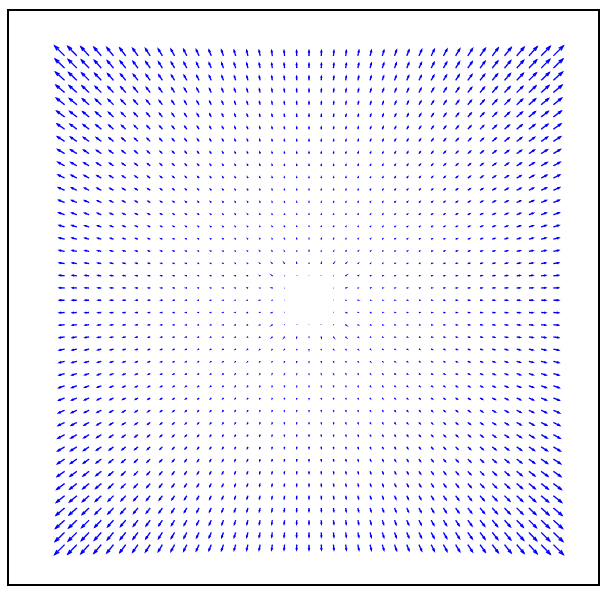
\includegraphics[scale=0.75]{images/radial_distortion.png}
\caption{Distribución de la distorsión radial de una imagen. Imagen tomada de: https://www.i-ciencias.com/pregunta/96683/que-es-el-tangencial-distorsion-de-opencv-en-realidad-tangencial .}
\label{fig:radial_distortion}
\end{figure}

Las \textit{Distorsiones tangenciales} son ocasionadas por no tener paralelas las lentes con el plano de la imagen, vea la distribución de la distorsión tangencial en la figura \ref{fig:tangential_distortion}. Para obtener expresiones que ayuden a corregir este tipo de distorsión se introducen dos parámetros: $p_{1}$ y $p_{2}$ dentro de las siguientes ecuaciones:
\[x_{corregida} = x + [2p_1y+p_2(r^2+2x^2)]\]
\[y_{corregida} = y + [p_1(r^2+2y^2)+2p_2x]\]

La estimación de los parámetros internos es importante en la calibración de las cámaras, de esto depende la exactitud de las mediciones de distancia dadas por la visión computacional. \cite{bradski2008learning}.

\begin{figure}
\centering
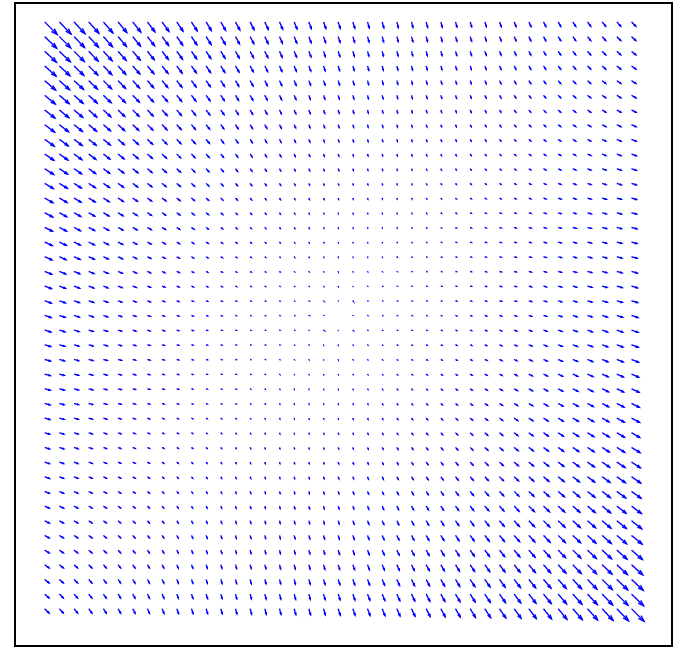
\includegraphics[scale=0.66]{images/tangential_distortion.png}
\caption{Distribución de la distorsión tangencial en una imagen. Imagen tomada de: https://www.i-ciencias.com/pregunta/96683/que-es-el-tangencial-distorsion-de-opencv-en-realidad-tangencial .}
\label{fig:tangential_distortion}
\end{figure}

Para poder hacer una corrección automática de todas las distorsiones, las herramientas de OpenCV (véase la sección 5.2) usan los cinco parámetros antes mencionados dentro de una matriz de 1x5 llamada \textit{matriz de coeficientes de distorsión}, en donde cada parámetro se acomoda de la siguiente forma:
\[[k_1 \quad k_2 \quad p_1 \quad p_2 \quad k_3]\]
	\section{Los espacios de color RGB y HSV}
El el pocesamiento de imágenes se usa el color debido a que es un buen descriptor para la identificación de objetos (mejor que otro tipo de segementación como el de escala de grises) \cite{gonzalez2002digital}.
		\subsection*{Percepción del color}
Según \cite{agoston2005computer} en el caso más simple, la percepción del color tiene tres características principales llamadas \textit{matiz, saturación y brillo}. 
\begin{itemize}
\item \textit{Matiz (Hue):} La matiz es un descriptor de qué tan combinados están los colores unitarios entre sí (si se entiende por color unitario a los colores rojo, amarillo, verde y azul).

\item \textit{Saturación (Saturation): } La saturación es la percepción de la relativa carga de color que tiene la matiz. Se puede decir que la saturación es una medida de qué tan puro es un color si éste es diluido en blanco.

\item \textit{Brillo: (Brightness)} El brillo es un atributo de la iluminación en la cual un objeto no aislado se ve afectado, es notable cuando un objeto de un  mismo color cambia su tonalidad debido a las variaciones de iluminación de su entorno.
\end{itemize}
		\subsection*{Espacios de color}
El \textit{espacio de color} es un modelo utilizado para facilitar la especificación de cualquier color de una manera estandarizada. Uno de los sistemas más conocidos, es el espacio de color RGB (por sus siglas en inglés red, green y blue), que está basado en un sistema coordenado ortogonal (como se observa en la Figura 2.3) en donde la escala de los colores primarios está cada uno en los ejes.

El espacio de color \textit{HSV (Hue-Saturation-Value)} es especificado por tres números que corresponden a la matiz (Hue), saturación (saturation) y el valor (value). La matiz corresponde a un ángulo de 0 a 360 grados. La saturación se toma entre valores de 0 a 1 que miden la salida de la matiz del blanco. El valor (value) que va del 0 al 1 mide la salida de la matiz del negro o \textit{color de energía cero}, véase la Figura 2.4 en donde se observa el modelo tridimencional de este espacio.

\begin{figure}
	\centering		
	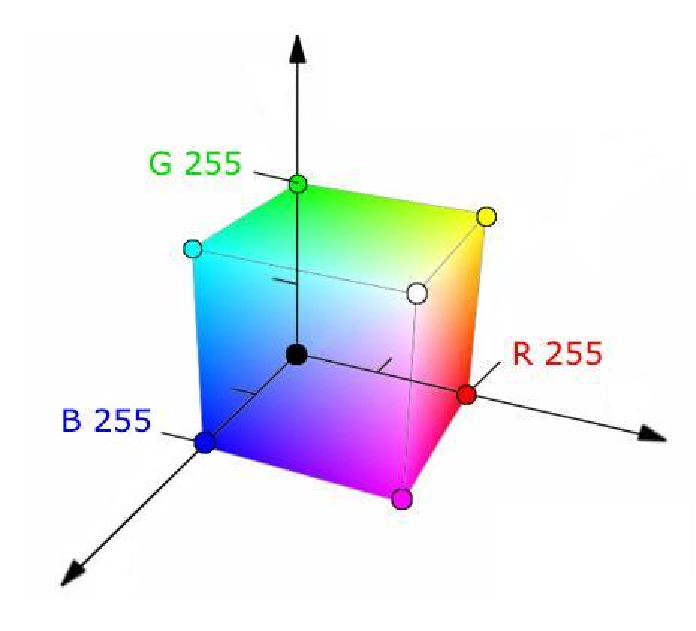
\includegraphics[scale=0.8]{images/RGB_model.pdf}
	\caption{Modelo tridimensional del espacio de color RGB. Imagen tomada de: https://lpurpura.wordpress.com/2011/05/03/modo-de-color/ .}		
\end{figure}

\begin{figure}
	\centering		
	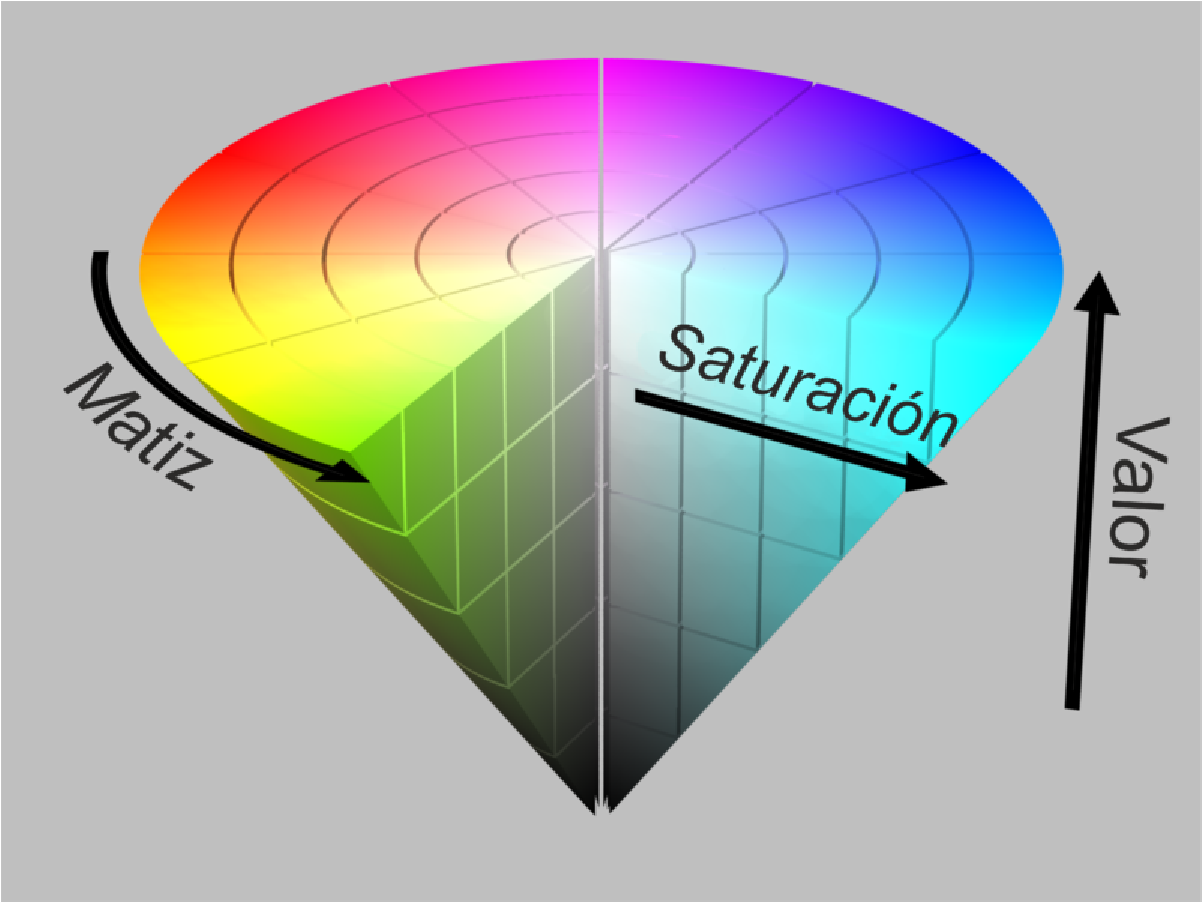
\includegraphics[scale=0.4]{images/hsv_space.pdf}
	\caption{Modelo tridimensional del espacio de color HSV. Imagen tomada de: $https://es.wikipedia.org/wiki/Modelo_-de_-color_-HSV$ .}		
\end{figure}

Tanto el espacio de color RGB y el HSV pueden representar la totalidad de los colores del espectro de luz visible, no obstante para el procesamiento de imágenes se utiliza el HSV ya que es una forma más sencilla para segmentar colores y es una forma más parecida a la que los seres humanos percibimos los colores.

	\section{Operadores morfológicos}	
La gran mayoría de las veces, cuando se hace procesamiento de imágenes, se necesitan ciertos procesos para eliminar el ruido circundante y dejar al elemento de interés aislado. Los \textit{operadores morfológicos} (erosión y dilatación) se pueden usar para este propósito.

Los \textit{operadores morfológicos} son operadores matemáticos basados en la forma de una imagen comunmente binaria (con pixeles blancos y negros) y sirven para preservar sus características y eliminar las irrelevancias. Dado que toda imagen está compuesta por pixeles, se pueden crear ciertos conjuntos de pixeles dentro de un vector para así poder aplicar operaciones matemáticas. 

La \textit{erosión} es el primer operador que se aplica cuando se desea eliminar el ruido en una segmentación, eso es porque elimina una gran cantidad de pixeles que tienden a tener mucha menor área que la figura de interés. Para lograr esto se establecen dos conjutos (de coordenadas de pixeles) $A$ y $B$. Si $A$ y $B$ son conjuntos dentro de un espacio euclidiano de N elementos, entonces la erosión de $A$ por $B$ es el conjunto de elementos $x$ para el cual $x + b \in  A$ para cada $b \in B$. Por lo tanto, de una manera más formal, la operación de erosión se puede definir con la expresión \ref{eq:erosion}.
En la figura \ref{fig:erosion_diagram} se puede observar de una manera más visual cómo funciona la operación de erosión dentro de una imagen binaria.
\begin{equation}
A\thinspace\ominus\thinspace B\thinspace=\thinspace \left \{ x \in E^N  \mid x+b \in A \enspace \forall \; b \in B\right \}
\label{eq:erosion}
\end{equation}

 Para entender de mejor manera cómo es esta operación se debe entender lo que es un \textit{kernel}. Un \textit{kernel} es un conjunto de pixeles de cualquier forma o tamaño que se caracteriza por tener un pixel de anclaje dentro de sí (en la figura \ref{fig:erosion_diagram} es el pixel con un punto blanco). En el ejemplo de la figura \ref{fig:erosion_diagram} se le llamará \textit{kernel} al conjunto $B$ y siempre debe ser de menor tamaño que el conjuto $A$. La intersección del conjunto $A$ con el $B$ al ir colocando el pixel de anclaje en cada pixel del conjunto $A$ es la imagen resultante para la erosión.
 
\begin{figure}
\centering 
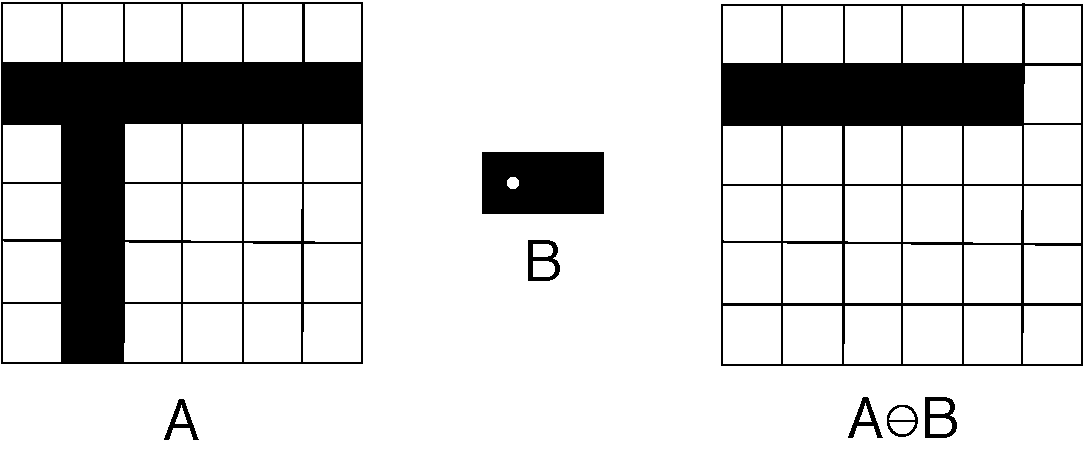
\includegraphics[scale=0.7]{images/erosion_diagram.pdf}
\caption{Ejemplo de la operación de erosión en una imagen binaria.}
\label{fig:erosion_diagram}
\end{figure}

En la figura \ref{fig:erosion_example} se ve que la erosión ha eliminado el ruido y la imagen se ve más limpia de puntos blancos que rodean la región de interés. El problema de hacer este procedimiento es que la imagen original suele verse afectada y tiende a encogerse o a deformarse, esto puede representar un problema para la detección de contornos. Para solucionarlo se procede a aplicar una operación opuesta a la erosión, mejor conocida como \textit{dilatación}.

Una vez eliminado el ruido gracias a la erosión, la \textit{dilatación} procede a ensanchar la figura de interés utilizando la adición de dos conjuntos de elementos. De la misma manera en que se hizo la erosión se procede a nombrar dos conjuntos $A$ y $B$. Si $A$ y $B$ son conjuntos dentro de un espacio euclidiano de N elementos. Sean $a \in A$ y $b \in B$ en donde $a=(a_1, ... ,a_n)$ y $b=(b_1,...,b_n)$, es decir conjuntos con coordenadas de pixeles, entonces la dilatación de $A$ por $B$ es el conjunto de todas las posibles sumas de elementos, de $A$ y $B$. De forma formal se expresa como \ref{eq: dilation}.
\begin{equation}
A\thinspace\oplus\thinspace B\thinspace=\thinspace \left \{ c \in E^N  \mid c=a+b \quad\forall \quad a \in A \; y\; \; b \in B\right \}
\label{eq: dilation}
\end{equation}


\begin{figure}
\centering
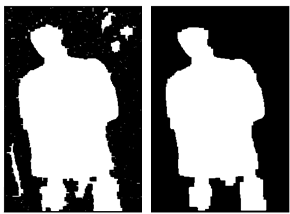
\includegraphics[scale=1]{images/erosion_example.png}
\caption{Eliminación de ruido alrededor de una figura de interés usando la erosión.  Imagen tomada de: $https://docs.opencv.org/3.4/d9/d61/tutorial_-py_-morphological_-ops.html$ .}
\label{fig:erosion_example}
\end{figure}

En la figura \ref{fig:dilation_diagram} se puede imaginar que si se coloca el \textit{kernel} dentro de los pixeles pertenecientes al conjunto $A$ y se suman, queda como resultado de $A \oplus B$ una imagen ensanchada, lo que puede ayudar a que la figura erosionada tenga mayor parecido a la imagen original \cite{4767941}. En la figura \ref{fig:dilation_example} está un ejemplo de cómo se ensancha una figura al aplicar la dilatación.

\begin{figure}
\centering
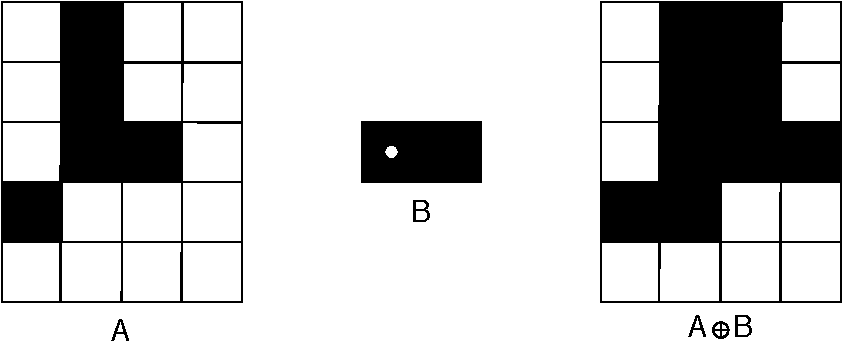
\includegraphics[scale=1]{images/dilation_diagram.pdf}
\caption{Ejemplificacion de la operación de dilatación en una imagen binaria.}
\label{fig:dilation_diagram}
\end{figure}

\begin{figure}
\centering
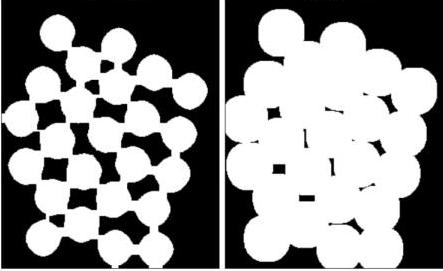
\includegraphics[scale=0.7]{images/dilation_example.jpg}
\caption{Ejemplificación de la dilatación aplicada en una segmentación de color. Imagen tomada de: $https://unipython.com/segmentacion-imagenes-algoritmo-watershed/$ .}
\label{fig:dilation_example}
\end{figure}